\documentclass[a4paper, 11pt]{article}
\usepackage{comment} % enables the use of multi-line comments (\ifx \fi) 
\usepackage{fullpage} % changes the margin
\usepackage{enumitem}
\usepackage[T1]{fontenc}
\usepackage[polish]{babel}
\usepackage[utf8]{inputenc}
\usepackage{ragged2e}
\usepackage{graphicx}
\usepackage{datatool}
\usepackage{rotating}
\usepackage{placeins}
\usepackage{pdflscape}
\usepackage{float}
\usepackage{listings}
\usepackage{xcolor} % for setting colors

\usepackage{color}

\usepackage{hyperref}
\hypersetup{
colorlinks,
citecolor=black,
filecolor=black,
linkcolor=black,
urlcolor=black
}

\definecolor{dkgreen}{rgb}{0,0.6,0}
\definecolor{gray}{rgb}{0.5,0.5,0.5}
\definecolor{mauve}{rgb}{0.58,0,0.82}


\lstset{frame=tb,
language=[sharp]C,
aboveskip=3mm,
belowskip=3mm,
showstringspaces=false,
columns=flexible,
basicstyle={\small\ttfamily},
numbers=none,
numberstyle=\tiny\color{gray},
keywordstyle=\color[HTML]{EA1212},
commentstyle=\color{dkgreen},
stringstyle=\color{blue},
breaklines=true,
breakatwhitespace=true,
tabsize=3,
otherkeywords={},
morekeywords={}
}


\title{Raport z wykonania ćwiczenia EntityFramework, LINQ2Entities}
\author{Jakub Płotnikowski}
\date{Listopad 2019r.}

\begin{document}

    \maketitle
    \tableofcontents
    
    \newpage
    
    \section{Kod źródłowy}
    
    \subsection{Definicja klasy Category}
    \lstinputlisting{resources/Category.cs}

    \subsection{Definicja klasy Product}
    \lstinputlisting{resources/Product.cs}
    
    \newpage
    
    \subsection{Definicja klasy Customer}
    \lstinputlisting{resources/Customer.cs}
    
    \subsection{Definicja klasy Order}
    \lstinputlisting{resources/Order.cs}
    
    \newpage
    
    \subsection{Definicja klasy ProdContext}
    \lstinputlisting{resources/ProdContext.cs}
    
    \subsection{Definicja funkcji AddCategory}
    \lstinputlisting{resources/AddCategory.cs}
    
    \subsection{Definicja funkcji AddProduct}
    \lstinputlisting{resources/AddProduct.cs}
    
    \subsection{Definicja całej klasy Program}
    \lstinputlisting{resources/Program.cs}

    
    \section{Bindowanie danych do komórek}

    \subsection{Wygląd formularza CategoryForm}
    \begin{center}
        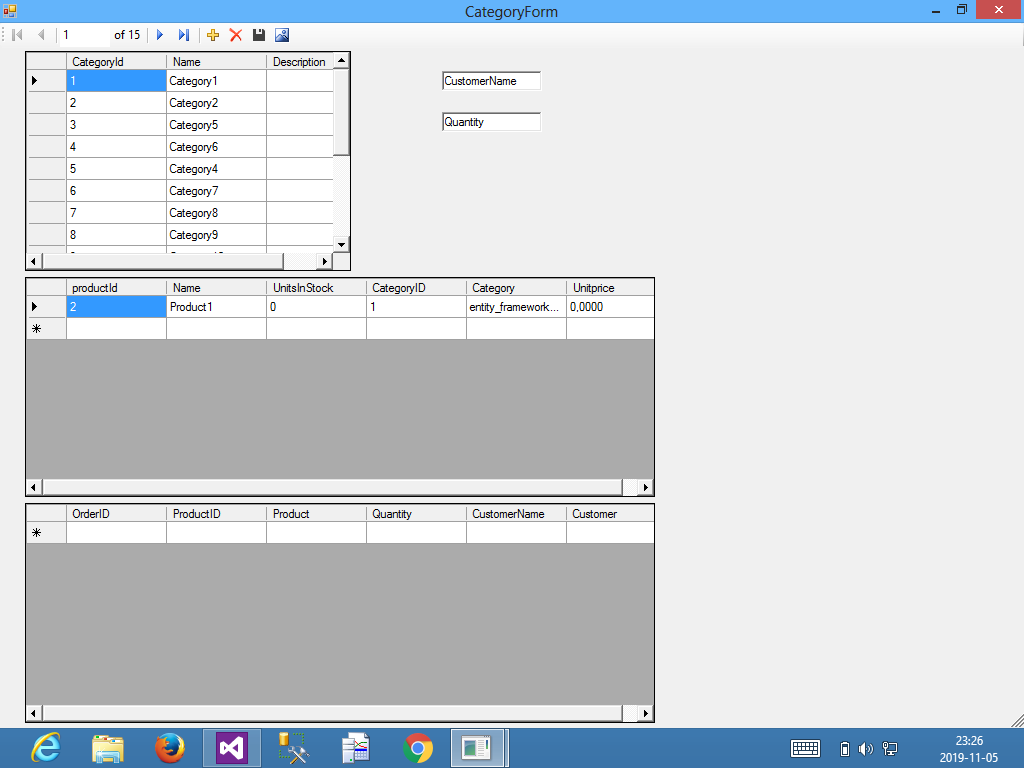
\includegraphics{images/CategoryForm1.png}
    \end{center}
    
    \newpage

    \subsection{Ustawienie pola CategoryID jako pole wyłącznie do odczytu}
    \lstinputlisting{resources/SetCategoryIdReadOnly.cs}
    
    \subsection{Ustawienie pola ProductId jako pole wyłącznie do odczytu}
    \lstinputlisting{resources/SetProductIdReadOnly.cs}


    \subsection{Metoda Load formularza CategoryForm}
    \lstinputlisting{resources/OnLoadMethod.cs}
    
    \newpage
    
    \subsection{Wynik działania, gdy klikniemy jakąś kategorię}
    
    W formularzu produktów pokażą się produkty, które należą do danej kategorii
    
     \begin{center}
        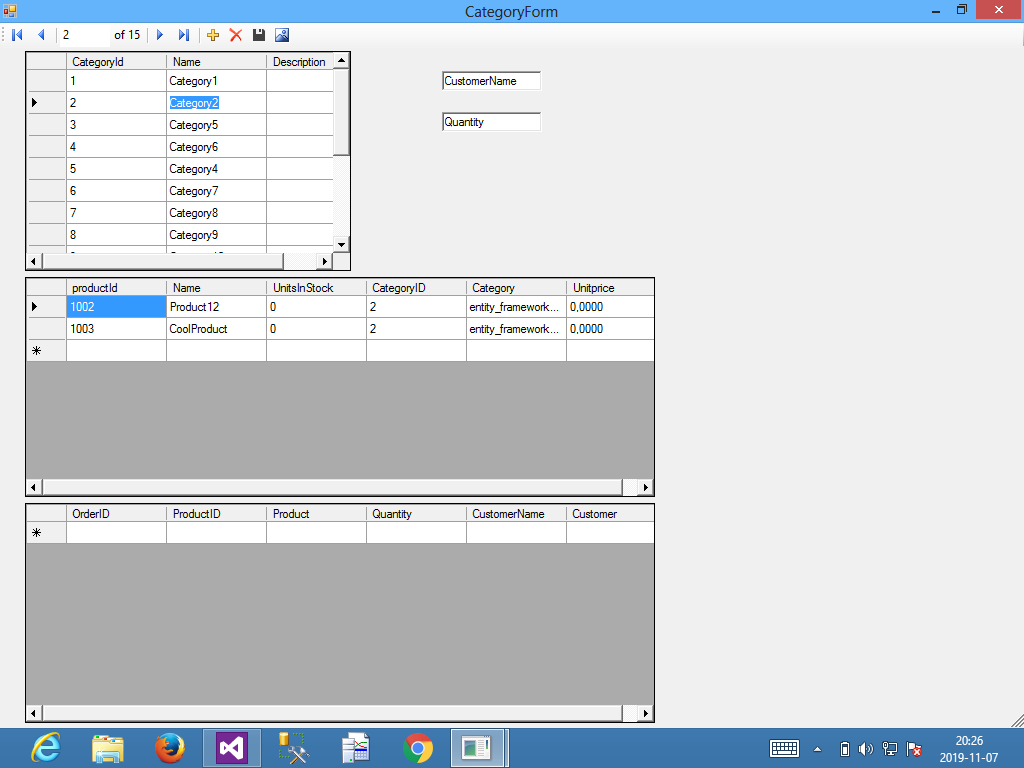
\includegraphics{images/CategoryForm3.png}
    \end{center}
    
    \newpage
    
    \section{Method syntax vs query syntax}
    
    \subsection{Widok wszystkich kategorii z bazy}
    
     \begin{center}
        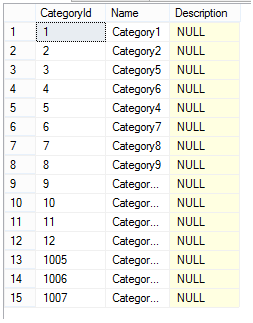
\includegraphics{images/SelectFromCategory.png}
    \end{center}
    
    \subsection{Widok wszystkich produktów z bazy}

    \begin{center}
        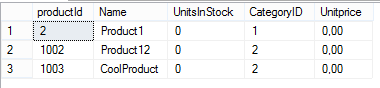
\includegraphics{images/SelectProduct.png}
    \end{center}
    
    \newpage
    
    \subsection{Wypisanie kategorii i produktów (różne sposoby)}
    
    \lstinputlisting{resources/ShowCategoriesAndProducts.cs}

    \lstinputlisting{resources/ShowAllAvailable.cs}

    \newpage
    
    \section{Dodawanie nowych zamówień}
    
    \subsection{Definicja metody onAddOrderClick oraz metod pomocniczych}
    
    Fragment klasy CategoryForm.cs
    
    Po walidacji odpowiednich textBoxów umożliwia dodanie zamówienia do bazy danych.
    
    \lstinputlisting{resources/OnAddOrderClick.cs}
    
    \subsection{Opis sposobu działania widoku}
    
    Widzimy 2 textBoxy, które należy uzupełnić odpowiednimi danymi.
    Po kliknięciu przycisku save, widzimy podane zamówienie w formularzu zamówień.
    
    \newpage

    \subsection{Widok dodawania zamówienia:}
    
    \begin{center}
        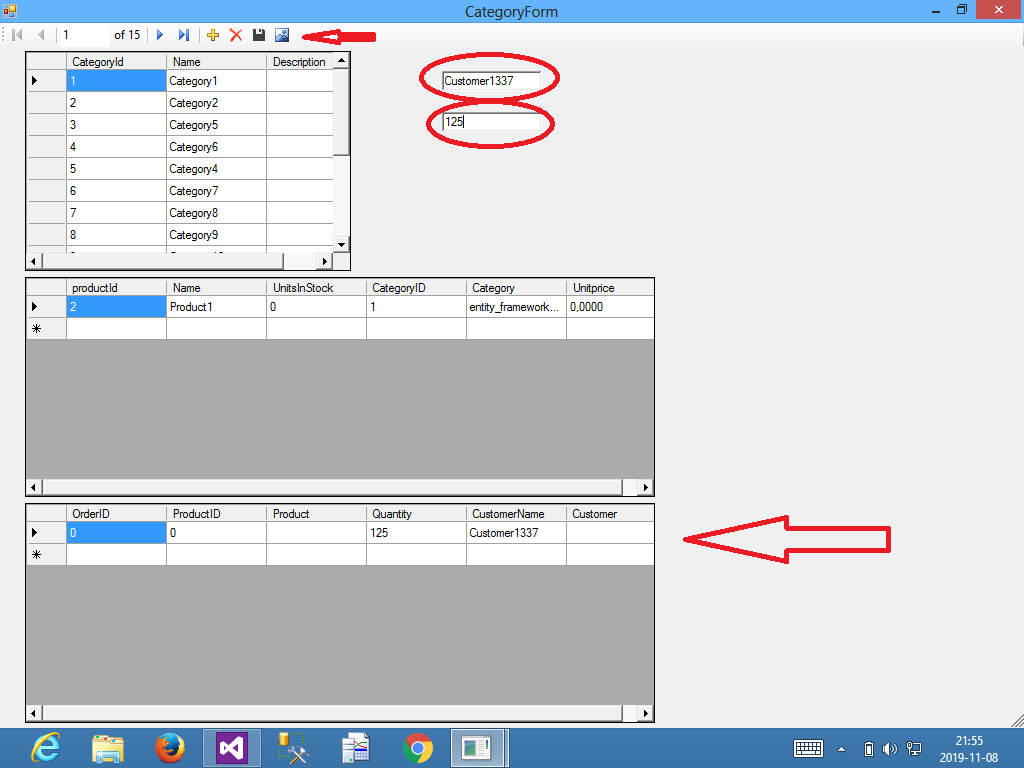
\includegraphics{images/AddOrder.png}
    \end{center}
    
    \newpage
    
    
    \section{Wykonanie migracje}
    
    \lstinputlisting{resources/Migration_AddCustomer.cs}
    \lstinputlisting{resources/Migration_AddDescription.cs}
    
    \newpage
    
    \lstinputlisting{resources/Migration_AddOrder.cs}
    
    \newpage
    
    \lstinputlisting{resources/Migration_AddUnitprice.cs}
    
    \newpage
    
    \lstinputlisting{resources/Migration_InitialCreate.cs}
    
    \newpage

    \section{Kod CategoryForm.cs oraz CategoryForm.Designer.cs}
    
    \lstinputlisting{resources/CategoryForm.cs}
    
    \newpage
    
    \lstinputlisting{resources/CategoryForm.Designer.cs}


    
    
\end{document}